\documentclass[12pt]{article}
\usepackage[hidelinks]{hyperref}    
\usepackage[all]{hypcap}   
\usepackage{graphicx}
\usepackage{amsmath}
\usepackage{xcolor}
\graphicspath{{../images/}}
\author{Andrea Malvezzi}
\title{\textbf{Architettura degli Elaboratori~-~Rappresentazione dell'informazione}}
\date{04 Ottobre, 2024}
\author{Andrea Malvezzi}
\begin{document}
\maketitle
\pagebreak
\tableofcontents
\pagebreak
\section{Codifiche e sistemi di numerazione}
I calcolatori elaborano tipi diversi di informazioni, ma alla base di ognuna di queste categorie ci sono i bit della memoria, ovvero dei valori binari.\\
Per convertire i dati dalla loro "forma originale" a un qualcosa di comprensibile dal calcolatore (ovvero sequenze di zero e di uno), occorre una codifica.
\subsection{Sistemi di numerazione posizionali}
Una codifica ha una \textbf{base} $b$, a cui corrisponde un quantitativo di caratteri con cui codificare i valori da convertire in un certo formato.\\
Ad esempio, la codifica binaria ha base $2$, in quanto utilizza solamente lo $0$ e l'$1$.\\
Altre codifiche importanti sono quella ottale (base 8) ed esadecimale (base 16, dal 9 in poi si usano le lettere in ordine alfabetico).
\subsection{Leggere un numero in una certa base}
Avendo un numero codificato in base $b$, allora tale numero corrisponderà a:
\begin{equation}
    \sum_{i=0}^{k} d_i \cdot b^i    \label{formula:leggere_codifica}    
\end{equation}
\subsubsection{Esempio di diversi tipi di codifica}
Prendiamo come esempio il numero 2001 in base decimale (quella con cui siamo abituati a contare nella matematica "standard").\\
Ora convertiamolo in binario, ottale e esadecimale:
\[
    2001_{10} = 11111010001_2
\]
In quanto il primo uno corrisponde a $1*2^{10}$, il secondo a $1*2^9$, e così via, fino all'ultimo che corrisponde a $1*2^0$, quindi a 1.
\[
    2001_{10} = 3721_8
\]
\[
    2001_{10} = 7D1_{16}
\]
Tutte queste 3 codifiche sono \textbf{equivalenti}, in quanto rappresentano tutte lo stesso numero.
\subsection{Metodi alternativi per effettuare conversioni}
Per convertire un numero in binario da decimale, basta dividerlo per 2 e segnare i resti:
\begin{gather*}
    2999 : 2 = 1499, \text{ con resto pari a } 1.\\
    1499 : 2 = 749, \text{ con resto pari a } 1.\\
    \text{etc} \dots \\
    5 : 2 = 2, \text{ con resto pari a } 1\\
    2 : 2 = 1, \text{ con resto pari a } 0
\end{gather*}
Mentre per fare la conversione inversa, si può optare per un metodo più alternativo, ovvero quello delle \textbf{moltiplicazioni successive}:
\begin{figure}[!htb]
    \centering
    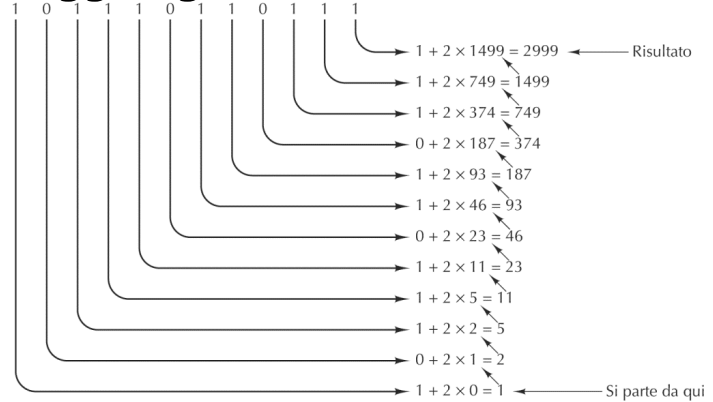
\includegraphics[width=.9\linewidth,height=.40\textheight,keepaspectratio]{rappresentazione_dati/mult_succ.PNG} % essenzialmente resiza l'immagine
    \begin{center}
        \caption{\label{fig:moltiplicazioni_successive}Partendo da sx e con un moltiplicatore pari a 0, per ogni cifra si somma la cifra in questione al doppio del moltiplicatore, per poi assegnare al moltiplicatore valore pari a quello appena ottenuto.}
    \end{center}
\end{figure}
\section{Numeri binari negativi}
Per codificare i numeri binari negativi si possono usare diverse tecniche, tra cui:
\subsection{Modulo e segno}
Si usa il bit più significativo (a sx) come segno, dove 0 indica il "+" e l'1 indica il "-".
\subsubsection{Esempio}
Usando 8 bit:
\begin{itemize}
    \item $6_{10} = \colorbox{yellow}{0}0000110_2$, dove il bit evidenziato indica il segno "+";
    \item $-6_{10} = \colorbox{yellow}{1}0000110_2$, dove il bit evidenziato indica il segno "-".
\end{itemize}
\subsection{Complemento a 1}
Qualora il numero da rappresentare fosse negativo, si complementa il modulo della codifica binaria di tale numero.
\subsubsection{Esempio}
\begin{itemize}
    \item $6_{10} = \colorbox{yellow}{0}0000110_2$;
    \item $-6_{10} = \colorbox{yellow}{1}1111001_2$, dove semplicemente si invertono i numeri dopo al bit di segno del 6.
\end{itemize}
\subsection{Complemento a 2}
Come il complemento ad 1, ma se il numero è negativo aggiunge anche un 1 in seguito all'operazione di complemento.
\subsubsection{Esempio}
\begin{itemize}
    \item $6_{10} = \colorbox{yellow}{0}0000110_2$;
    \item $-6_{10} = \colorbox{yellow}{1}11110\colorbox{green}{10}_2$, dove guardando il secondo esempio del completamento a 1, è facile notare la differenza tra le due (le cifre evidenziate in verde).
\end{itemize}
\subsection{Codifica in eccesso}
Un altro modo per rappresentare un numero consiste nel definire un "\textbf{offset}" o \textbf{eccesso} da aggiungere al valore del numero che si vuole rappresentare.\\
Di conseguenza, i numeri negativi diventeranno più piccoli, mentre quelli positivi più grandi.
\subsubsection{Esempio teorico}
Volendo rappresentare i numeri nell'intervallo $[-2^{k-1}, 2^{k-1}-1]$, potremmo decidere di sommare a tutti i valori corrispondenti a tali numeri $2^{k-1}$. In questo modo avremmo:
\begin{gather*}
    000 \dots 0 = -2^{k-1}\\
    111 \dots 1 = 2^{k-1}-1\\
    100 \dots 0 = 0\\
\end{gather*}
\subsubsection{Esempio pratico}
Voglio rappresentare $2^5-1$ valori con eccesso di 4. Ovviamente serviranno 5 bit totali per questa operazione in quanto $2^5-1 = 31$ cifre, più lo $0$ quindi $32$ totali. Perciò:
\[ -16_{10} \Rightarrow -16 + 4 = -12 \]
Ora, essendo il numero trattato negativo, trasformiamo il suo valore assoluto in binario, usando 5 bit:
\[ |-12|_{10} = 01100_2 \]
In seguito, essendo il numero da convertire negativo, occorerà applicare la codifica di completamento a 2 alla conversione in binario ottenuta precedentemente:
\[ 01100_2 \Rightarrow 10011_2 + 00001_2 \Rightarrow 10100_2 \]
Rappresentiamo ora l'11:
\[11_{10} + 4_{10} = 15_{10} = 01111_2\]
\subsection{Codifica floating point}
La codifica \textbf{floating point} si basa sul rappresentare un numero $n$ tramite altri due numeri: un $f$ detto \textbf{mantissa} e un $e$ detto \textbf{esponente}.\\
La mantissa può essere normalizzata (la prima cifra non può essere $0$), oppure no, in base alle caratteristiche della codifica con cui si sta operando.
\subsubsection{Esempio di codifica con normalizzazione}
Supponiamo di operare con una codifica con normalizzazione, offset pari a 64 e base 2. Volendo rappresentare il numero 432:
\begin{center}
    Convertiamo 432 in binario:
\end{center}
\[432_{10} = 110110000_2\]
\begin{center}
    Ora posizioniamo la virgola (o il punto) dopo alla prima cifra della parola ottenuta:
\end{center}
% TODO: chiedi spiegazioni al prof su come effettuare il passaggio da n a floating point
\[110110000_2 \Rightarrow 1.10110000_2\]
\begin{center}
    Contando i numeri dopo alla virgola, otterremo i bit dell'esponente, da sommare con l'offset per ottenere la cifra effettiva da convertire in binario:
\end{center}
\[8 + 64 = 72_{10} \Rightarrow 1001000_2\]
\section{Rilevazione e Correzione errori}
Quando si lavora con dei dati potrebbero riscontrarsi degli errori. Per rilevare ed eventualmente anche correggere tali errori si aggiungono dei bit detti di controllo davanti alla parola corrispondente al dato.
\subsection{Distanza di Hamming}
La distanza di Hamming tra due parole è il numero di bit di cui differiscono tra loro, ad esempio tra $0011$ e $1111$ vi è una distanza di $2$.\\
Per \textbf{rilevare} $n$ bit errati in una parola è necessario un codice con distanza di Hamming $\geq n + 1$.\\
Per \textbf{correggere} $n$ bit errati in una parola è necessario un codice con distanza di Hamming $\geq 2n+1$.
\subsection{Il bit di parità}
Uno dei codici per il controllo dell'errore più usati è quello del "Bit di parità".\\
Si ha un unico bit di controllo che si sceglie per rendere pari il numero di uno nella parola da controllare. Qualora il dato, una volta trasmesso etc$\dots$ non avesse un numero pari di 1, allora si potrà controllare i bit uno per uno per individuare l'errore.
\subsection{Correzione dell'errore con codice di Hamming}
Avendo una parola lunga $n_1$ bit e decidendo di aggiungervi $n_2$ bit di controllo dell'errore, allora il codice di Hamming sarà in grado di correggere tutti i possibili errori \textbf{su singoli bit} usando il numero minimo di bit di controllo $n_2$ che soddisfa la seguente disequazione:
\begin{equation}
    n_1 + n_2 + 1 \leq 2^{n_2} \label{eq:codice_Hamming}
\end{equation}
Questi bit di controllo (di parità) verranno posizionati nelle posizioni con indice pari alle potenze di 2, quindi alle posizioni $1, 2, 4, 8, 16, \dots$ e controlleranno proprio i gruppi corrispondenti a tali posizioni (vedi esempio seguente).
\subsubsection{Esempio di codice di Hamming}
A seguire un esempio di applicazione del codice di Hamming: qui si ha una parola di 16 bit, quindi occorerà trovare $n_2$ minimo per risolvere l'equazione (\ref{eq:codice_Hamming}). Quindi:
Prendiamo ad esempio $n_2$ pari a $4$:
\[16 + 4 + 1 \leq 2^{4} ? \text{ falso.}\]
Aumentiamo quindi $n_2$ e riproviamo:
\[16 + 5 + 1 \leq 2^{5} ? \text{ vero.}\]
Quindi avremo 5 bit di parità da posizione nelle posizioni $(1, 2, 4, 8, 16)$, ovvero:
\begin{figure}[!htb]
    \centering
    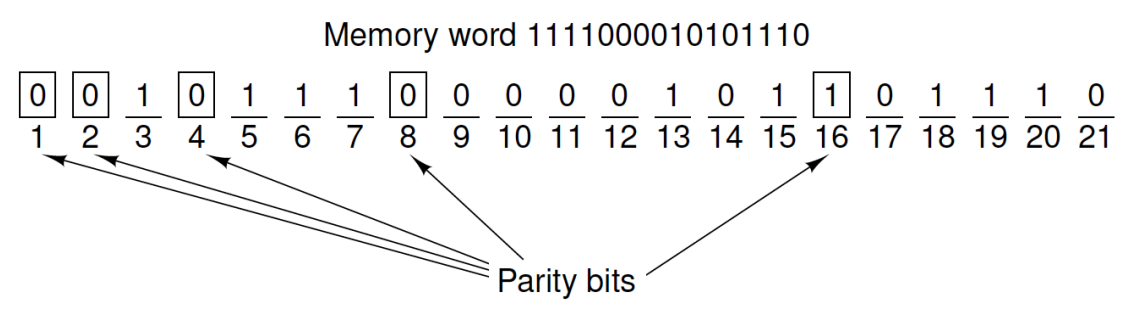
\includegraphics[width=1\textwidth, height=.7\textheight,keepaspectratio]{rappresentazione_dati/hamming_example.png} % essenzialmente resiza l'immagine
    \begin{center}
        \caption{\label{fig:esempio_Hamming}Qui il bit di parità nella posizione 4 controlla il numero di uni prima di tale posizione, ed essendocene solamente uno, viene posto pari a 0.} % label fuori da caption spesso non va, mettilo dentro
    \end{center}
\end{figure}\\
Per trovare la posizione dell'errore, occorre
\end{document}